\documentclass[11pt]{article}
\usepackage[utf8]{inputenc}
\usepackage[russian]{babel}
\usepackage[T1]{fontenc}
\usepackage{amssymb,amsmath,clrscode,graphicx,indentfirst}

\author{Олег Смирнов}
\title{Курс kiev-clrs -- Лекция 4. Сортировка Quicksort, рандомизированные алгоритмы}
\date{4 апреля 2009 г.}

\begin{document}
\maketitle
\tableofcontents

\newpage
\setlength{\parskip}{1ex plus 0.5ex minus 0.2ex}
\section{Цель лекции}
\begin{itemize}
\item Рассмотреть сортировку Хоара
\item Рассмотреть рандомизированные алгоритмы
\item Проанализировать алгоритм Хоара в классическом и в рандомизированном варианте
\end{itemize}

\section{Алгоритм Хоара: Quicksort}

Алгоритм входит в Top10 вместе с методом Монте-Карло, симплекс-методом и быстрым преобразованием Фурье.

Алгоритм вида "Разделяй и властвуй", сортировка делается "на месте", так же как сортировка вставкой в отличии от сортировки слиянием. Шаги алгоритма:
\begin{itemize}
\item Divide: деление массива на два подмассива относительно опорного элемента (pivot) $x$: элементы левого подмассива $\leqslant x$, правого $\geqslant x$
\item Conquer: рекурсивная сортировка двух подмассивов
\item Combine: тривиально
\end{itemize}
Проще говоря, Quicksort -- это рекурсивное деление, тогда как Mergesort -- рекурсивное слияние.

Ключевой частью алгоритма является процедуры Partition, которая выполняется за линейное время $(O(n))$:
\begin{codebox}
\Procname{$\proc{Partition}(A, p, q)$ \Comment $A[p \twodots q]$}
\li	$x \gets A[p]$	\Comment pivot
\li	$i \gets p$
\li	\For $j \gets p+1$ \To $q$
\li		\Do \If $A[j] \leqslant x$
\li		\Then $i \gets i+1$
\li			обменять $A[i] \iff A[j]$
		\End
	\End
\li	обменять $A[p] \iff A[j]$
\li \Return i
\End
\end{codebox}

\begin{figure}[ht]
  \centering
  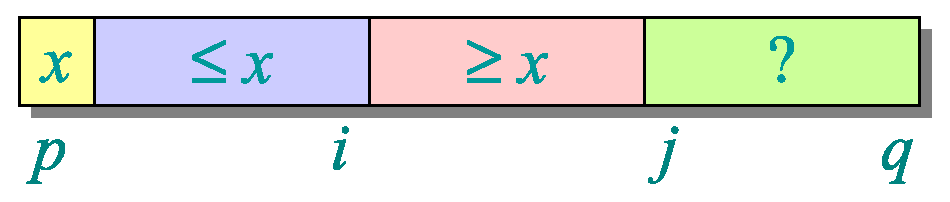
\includegraphics[width=3in]{lecture4/invariant.eps}
  \caption{Инвариант цикла}
  \label{fig:invariant}
\end{figure}

Доказательство инварианта (рис. \ref{fig:invariant}):
\nopagebreak
\begin{itemize}
\item Инициализация: в начале цикла инвариант выполняется, так как $i = p$ и $j = p+1$ 
\item Сохранение: если на очередном шаге $A[j] \geqslant x$, инвариант выполняется и счетчик $j$ увеличивается на единицу
\item Завершение: если $A[j] \leqslant x$, инвариант выполняется через обмен элемента $A[j]$ с $A[i]$ и сдвига границы левой части массива $i = i+1$
\end{itemize}

Алгоритм весьма прост для понимания. Время выполнения процедуры равно $O(n)$ для массива из $n$ элементов.
\begin{figure}[ht]
  \centering
  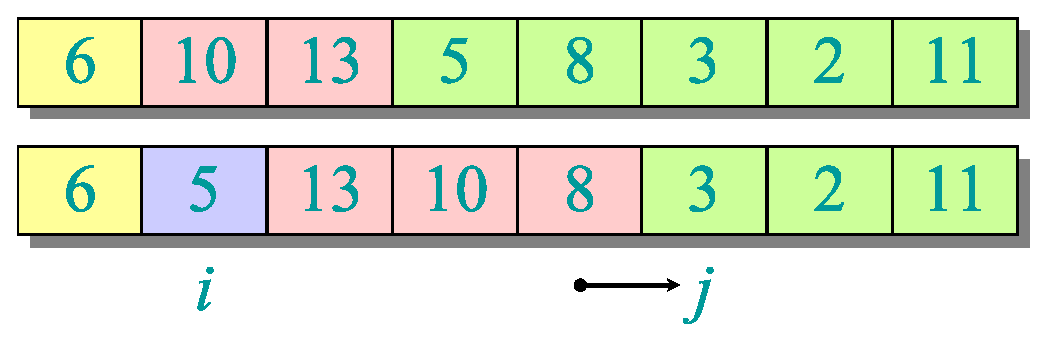
\includegraphics[width=3in]{lecture4/example1.eps}
  \caption{Пример работы}
  \label{fig:example1}
\end{figure}

Пример работы процедуры (рис. \ref{fig:example1}):
\begin{itemize}
\item шаге 0: $i$ на $6$, $j$ на $10$
\item шаге 1: обменеваются местами $10$ и $5$, $j$ на $8$
\item шаге 2: обменеваются $13$ и $3$, $i$ на $3$, $j$ на $2$
\item шаге 2: обменеваются $10$ и $2$, $i$ на $2$, $j$ на $11$
\item на последнем шаге опорный элемент перемещается на середину (вместо $2$) 
\end{itemize}
В конце работы элементы меньше или равные опорному находятся слева, остальные -- справа.

Алгоритм QuickSort:
\nopagebreak
\begin{codebox}
\Procname{$\proc{Quicksort}(A, p, q)$}
\li	\If $p < q$
\li		\Then $r \gets $ Partition(A, p, q)
\li			Quicksort(A, p, r-1)
\li			Quicksort(A, r+1, q)
	\End
\End
\end{codebox}

Начальные параметры вызова: Quicksort(A, 1, n)

Один из способов оптимизации Quicksort -- использования отдельной процедуры для маленьких массивов, например для $n \leqslant 5$ (например прямое сравнение). Также применяют хвостовую оптимизацию рекурсии.

\section{Анализ Quicksort}

Предположим, что все элементы различны, т.к. в случае дублирующихся элементов алгоритм работает более эффективно.

\subsection{Наихудший случай}

Легко видеть, что наихудшим образом алгоритм будет себя вести, если подпрограмма, выполняющая разбиение, порождает одну подзадачу с $n-1$ элементов, а вторую -- с $0$ элементов. Это происходит в том случае, если все элементы массива больше либо меньше выбранного опорного элемента.
\begin{align*}
  T(n) = \\
    = T(0) + T(n-1) + \Theta(n) \\ 
    = \Theta(1) + T(n-1) + \Theta(n) \\
    = T(n-1) + \Theta(n) \\
    = \Theta(n^2) \text{ (арифметическая прогрессия)}
\end{align*}

Дерево рекурсии для случая $T(n) = T(0) + T(n-1) + cn$ (рис. \ref{fig:tree1}). 
\begin{figure}[ht]
  \centering
  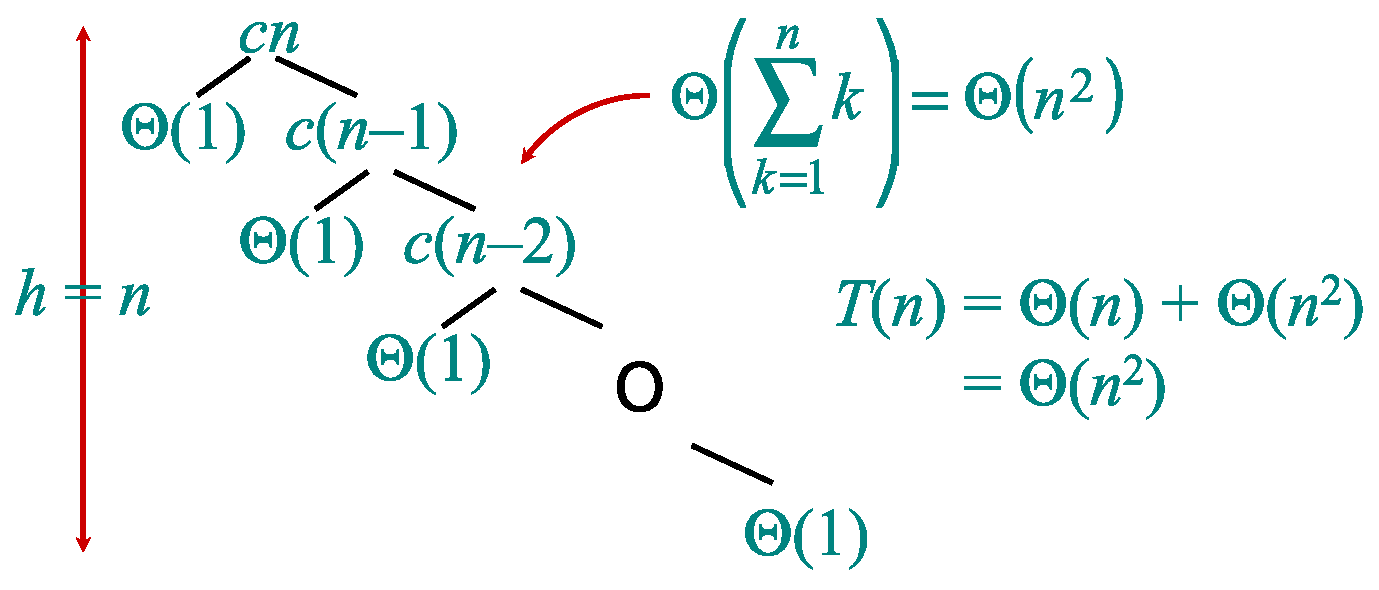
\includegraphics[width=3in]{lecture4/tree1.eps}
  \caption{Дерево наихудшего случая}
  \label{fig:tree1}
\end{figure}

Высота дерева $h = n$. Сумма правой ветви -- $\Theta(\sum_{k=1}ck) = \Theta(n^2)$, левых ветвей -- ${\Theta(1)}n$. Суммарное время работы в таком случае равно $T(n) = \Theta(n) + \Theta(n^2) = \Theta(n^2)$

\subsection{Наилучший случай}

Возникает, когда процедура делит массив на две равные части: $n/2$ и $n/2$. Время работы оценивается рекуррентностью:
\begin{equation*}
T(n) \leqslant 2T(\frac{n}{2}) + \Theta(n)
\end{equation*}
Согласно второму случае основного метода, ответ $T(n) = O(n \lg n)$

\subsection{Средний случай}

Рассмотрим "почти средний" случай. Предположим, что процедура всегда разбивает массив на части $\frac{1}{10}$ к $\frac{9}{10}$

Получим рекуррентость: $T(n) = T(\frac{1}{10} n) + T(\frac{9}{10} n) + \Theta(n)$. Построим дерево, явно вводя константу $c n$ вместо $\Theta(n)$.
\begin{figure}[ht]
  \centering
  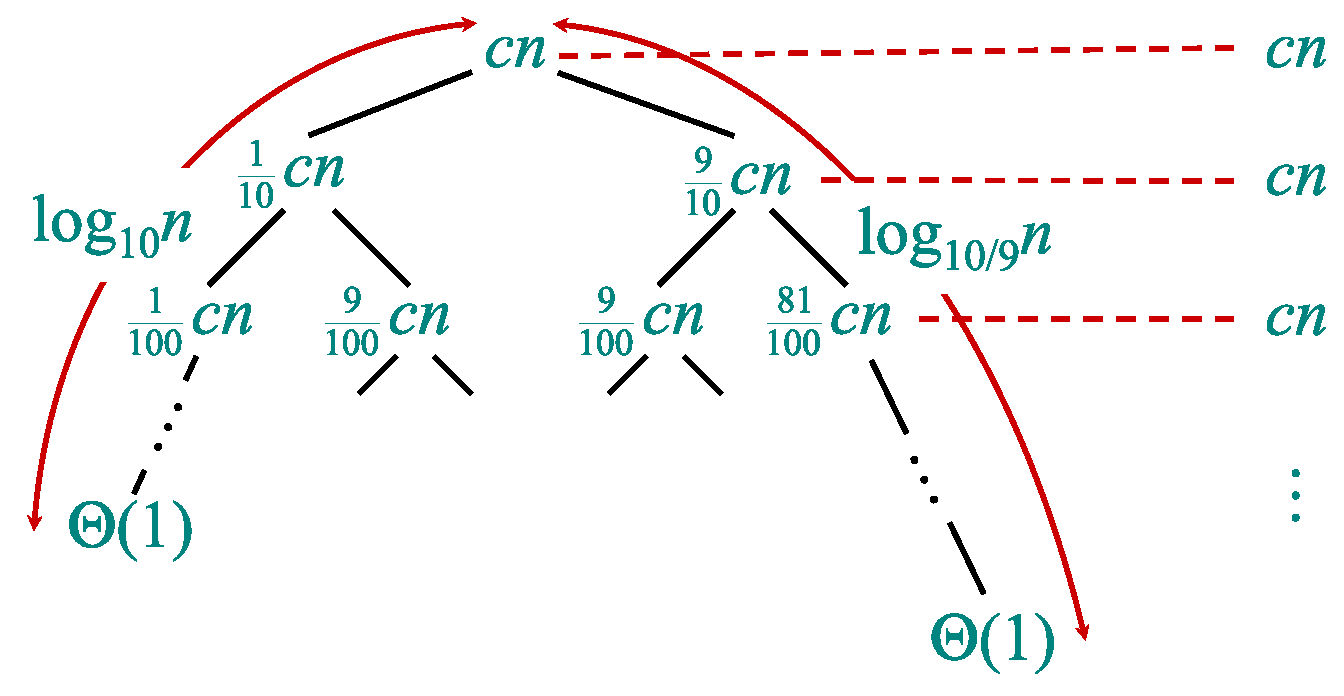
\includegraphics[width=3in]{lecture4/tree2.eps}
  \caption{Дерево "почти среднего" случая}
  \label{fig:tree2}
\end{figure}

Время работы каждого уровня дерева будет $\leqslant c n$. Глубина дерева будет разной для левой и правой ветви (рис. \ref{fig:tree2}). В левой части $\log_{10} n$, в правой $\log_{\frac{10}{9}} n$
\begin{align*}
  T(n) \leqslant \\
    \leqslant c n \log{\frac{10}{9}} + \Theta(n) = \\
    = O(n \lg n)
\end{align*}

\begin{align*}
  T(n) \geqslant \\
    \geqslant c n \log{10} + \Theta(n)
\end{align*}

Таким образом, $T(n) = \Theta(n \lg n)$

Т.е., несмотря на то, что разбиение в соотношении один к девяти выглядит довольно несбалансированным, в асимптоптическом пределе алгоритм ведет себя так же, как и при делении задачи на две равные части. Фактически, даже разбиение девяносто девять к одному даст время работы алгоритма $O(n \lg n)$. Причина в том, что любое разбиение, характеризующееся конечной \emph{константной} пропорциональности, приводит к образованию рекурсивного дерева высотой $\Theta(\lg n)$ и временем работы каждого уровня $O(n)$. Время работы алгоритма будет составлять $O(n \lg n)$.

Предположим, что процедура поочередно генерирует ``хорошие'' и ``плохие'' разбиения.

В ``хорошем случае'': $L(n) = 2U(\frac{n}{2}) + \Theta(n)$

В ``плохом случае'': $U(n) = L(n-2) + \Theta(n)$

Получаем систему уравнений, в которой граничные случае с константными данными опущены.
\begin{align*}
L(n) = \\
	= 2(L(\frac{n}{2} -1) + \Theta(\frac{n}{2})) + \Theta(n) = \\
	= 2L(\frac{n}{2} -1) + \Theta(n) = \\
	= \Theta(n \lg n) \text{ (по основному методу)}
\end{align*}

\section{Рандомизированные алгоритмы}

Предположим, компания хочет взять на работу нового программиста. Согласно договоренности, 
агентство должно присылать работодателю по одному кандидату в день. HR проводит с каждым
собеседование, после чего принимает решение, брать его на работу или нет. За каждого
направленного кандидата компания платит агентству некоторую сумму. Однако наем выбранного
кандидата на работу фактически стоит дороже, поскольку при этом необходимо уволить
предыдущего сотрудника, а также уплатить агентству более значительную сумму за выбранного кандидата.

Компания пытается сделать так, чтобы должность всегда занимал наиболее достойный из всех
кандидатов. Как только квалификация очередного претендента окажется выше квалификации
существующего, он будет уволен, а его место займет более подходящий кандидат.
Работодатель готов понести все необходимые расходы, но хочет оценить, во что обойдется ему
подбор нового сотрудника. 

Процедура Hire описывает алгоритм найма в виде псевдокода:
\begin{codebox}
\Procname{$\proc{Hire}(n)$}
\li	Best $ \gets 0$
\li	\For $i \gets 1$ \To $n$
\li		\Do Собеседование с кандидатом $i$
\li			\If кандидат $i$ лучше Best
\li				\Then Best $ \gets i$
\li				Нанимаем кандидата $i$
				\End
			\End
		\End
	\End
\end{codebox}

Пусть стоимость собеседования равна $c_i$, а стоимость найма -- $c_h$. Пусть $m$ -- количество
нанятых сотрудников. Тогда полная стоимость, затраченная при работе этого алгоритма, равна $O(n c_i + m c_h)$.

Очевидно, что в интересах агенства максимизировать $m$, а в интересах компании -- минимизировать.

Одним из способов избежать наихудшего случая, когда $m = n$, является рандомизация -- контроль
за распределением входных данных.

\section{Вероятностный анализ. Часть 1}

При анализе рандомизированных алгоритмов будет использоваться индикаторная случайная величина.
С помощью неё можно сделать удобный переход от вероятности к математическому ожиданию.
Пусть дано пространство выборки $S$ и событие $A$.
Тогда индикаторная случайная величина $I\{A\}$, связанная с событием $A$, определяется так:
\begin{equation*}
	I\{A\} = \begin{cases}
		1, \text{если событие $A$ произошло} \\
		0, \text{событие $A$ не произошло}
	\end{cases}
\end{equation*}

Пример использования: определим мат. ожидание того, что при подбрасывании монеты выпадет орел.
Пространство событий имеет вид $S = \{H, T\}$, где вероятность выпадения $Pr\{H\} = Pr\{T\} = \frac{1}{2}$.
Можно определить индикаторную величину $X_H$, связанную с событием $H$. Математическое ожидание того,
что выпадет орел, равняется мат. ожиданию индикаторной величины $X_H$:
\begin{align*}
	E[X_H] = E[I\{H\}\ = \\
	= 1 \cdot Pr\{H\} + 0 \cdot Pr\{T\} = \\
	= 1 \cdot (1/2) + 0 \cdot (1/2) = \\
	= 1/2.
\end{align*}

Полезная лемма: пусть событие $A$ принадлежит пространству событий $S$, и пусть $X_A = I\{A\}$. Тогда мат. ожидание
\begin{equation}
E[X_A] = Pr\{A\}
\end{equation}

Указание к доказательству: использовать определению мат. ожидания для случайной величины $E[X] = \sum_x x Pr \{X = x\}$

\section{Вероятностный анализ. Часть 2}

Необходимо оценить мат. ожидание события, соответствующего найму нового программиста. Пусть $X$ -- случайная величина, значение которое равно количеству наймов нового сотрудника. По определению мат. ожидания:
\begin{equation*}
E[X] = \sum_x x Pr\{X = x\}
\end{equation*}

Используем индикаторную величину:
\begin{equation*}
	X_i = I\{i\text{-й кандидат нанят}\} = \begin{cases}
		1, \text{если кандидат нанят} \\
		0, \text{если кандидат отклонен}
	\end{cases}
\end{equation*}
\begin{equation*}
X = X_1 + X_2 + \twodots + X_n
\label{l2}
\end{equation*}
Из леммы:
\begin{equation*}
E[X_i] = Pr\{i\text{-й кандидат нанят}\}
\end{equation*}
Вероятность того, что претендент с номером $i$ выше квалификации с номерами от 1 до $i-1$ равна $1/i$, т.о.
\begin{equation*}
E[X_i] = 1/i
\end{equation*}
Тогда:
\begin{align*}
	E[X] = E[\sum_i X_i] = \\
	= \sum_i E[X_i] = \\
	= \sum_i \frac{1}{i} = \text{ (гармоническое число)} \\ 
	= \ln n + O(1)
\end{align*}
Таким образом, если проведено интервью со всеми $n$ кандидатами, в среднем будет нанято $\ln n$ из них. Тогда полная стоимость найма будет составлять $\O(c_h \ln n)$.

\section{Рандомизированный Quicksort}

Исправить ситуацию с наихудшим случаем можно двумя способами: случайно перемешать элементы массива или случайно выбирать опорный элемент. Тогда:
\begin{itemize}
\item время выполнения не зависит от порядка элементов
\item не зависит от входного распределения
\item наихудший случай зависит только от характеристик генератора случайных чисел
\end{itemize}

Для реализации достаточно модифицировать процедуру разбиения:
\begin{codebox}
\Procname{$\proc{Randomized\_Partition}(A, p, r)$}
\li	$i \gets $ Random(p, r)
\li	обменять $A[i] \iff A[j]$
\li	\Return Partition(A, p, r)
\End
\end{codebox}

\section{Анализ рандомизированного Quicksort}

Легко показать, что в наихудшем случае время работы Randomized\_Quicksort равно $\Theta(n^2)$
\begin{align*}
T(n) = \max_{0 \leqslant q \leqslant n-1} (T(q) + T(n-q-1)) + \Theta(n)
\end{align*}

Параметр $q$ изменяется в интервале от 0 до $n-1$, поскольку на выходе Partition мы получаем
две подзадачи суммарным размером $n-1$. Предположим, что $T(n)$ ограничено сверху $cn^2$:
\begin{align*}
T(n) \leqslant \max_{0 \leqslant q \leqslant n-1} (cq^2 + c(n - q -1)^2) + \Theta(n) = \\
= c \cdot \max_{0 \leqslant q \leqslant n-1} (q^2 + (n-1-q)^2) +\Theta(n) \leqslant \\
\leqslant cn^2 - c(2n -1) + \Theta(n) \leqslant \\
\leqslant cn^2
\end{align*}
Т.е. $T(n) = O(n^2)$. Аналогично доказывается $T(n) = \Omega(n^2)$

Для среднего случая рандомизированной версии Quicksort когда все элементы во входном
массиве различны.

\end{document}
